\chapter{\label{ch:implementation_issues}Implementation Issues}
This chapter explains how we implemented our method and the different software and file types used.

% -------------------------------------------------------------
% Section
% -------------------------------------------------------------
\section{Joints and muscles}
To construct our model, we used the 3D animation software Autodesk Maya and MEL (Maya Embedded Language) scripting. As an initial basis, we used the polygonal skeleton model described in chapter \ref{ch:human_torso_model}; we then divided it into its constituent parts: ribs, sternum, vertebrae and intervertebral discs. These different parts were made rigid so that constraints can be applied to them; we have also assigned physiology-based masses using data given by \cite{dilorenzo2009breathing} (see table \ref{tab:body_masses}). In addition, we modelled the joints linking the different rigid parts as already detailed in chapter \ref{ch:human_torso_model}:

\begin{description}
\item[vertebrae (C1--C7, T1--T12, L1--L5):] ball joints whose centres are located at the middle of the segment defined by the centres of mass of adjacent vertebrae; simulating the intervertebral discs joint function.
\item[vertebrae (T1--T12) -- ribs (R1--R12):] hinge joints crossing the \emph{articular facets for the transverse processes of vertebrae} and the middle of the \emph{superior articular facet for the vertebral body} and the \emph{inferior articular facet for the vertebral body}.
\item[ribs (R1--R9) -- sternum:] spring joint simulating the cartilage.
\end{description}

Since the muscle model we used can only connect to the centre of a rigid object, boxes are attached to polygon vertices with a pin constraint (see figure \ref{fig:r2-r3_mus_joints}). To form the different muscles (rib cage and abdominal muscles) we adopted a procedural approach using MEL scripting: 

\begin{enumerate}
\item Boxes serving as nodes connecting one extremity of a muscle to the other are placed on the different rigid parts of the skeleton.
\item Each box is linked to a rigid part through a pin constraint.
\item The different muscles are added between the nodes.
\item The parameters of the muscles are tuned.
\end{enumerate}

For the abdominal cavity, we used a polygonal sphere whose centre is fixed in space but whose shape deforms due to the displacement of its vertices.

\begin{figure}
\centering
\subfigure[Muscle and joint structures between rib 2 and rib 3.]{
\includegraphics[height=0.45\textwidth]{pics/r2-r3_mus_joints}
\label{fig:r2-r3_mus_joints}
}
\subfigure[Muscle structure in the abdominal cavity.]{
\includegraphics[height=0.45\textwidth]{pics/abdo_box}
\label{fig:abdo_box}
}
\caption[Comparison with the simulated spine]{\subref{fig:r2-r3_mus_joints} muscle and joint structures between rib 2 and rib 3. Hinge joints (red) connect each rib and their associated vertebrae. The intercostal muscles are modelled as springs (green) and each muscle connects one node (blue box) to another. Each node is attached to a rib with a pin constraint (brown) at the center of mass of the ribs (points A and B). \subref{fig:abdo_box} the abdominal cavity is modelled as a polygonal sphere (brown) where nodes (blue) are attached to vertices. The abdominal muscles connect the different nodes (e.g. the diaphragm, in green, at the top of the cavity).}
\label{fig:mus_joints}
\end{figure}

% -------------------------------------------------------------
% Section
% -------------------------------------------------------------
\section{Abdominal movement}
From a modelling perspective, the vertices of the polygonal sphere used to simulate the abdominal cavity are passive at the bottom and the back side, while those on the diaphragm, the lateral and front parts, are active. At each frame, we compute the pressure force (see equation \ref{eq:pressure_force}) for each active vertex with MEL scripting and send the resulting impulse force as an input to the Runge Kutta Adaptive rigid solver. The solver displaces the vertices according to the given impulse and the muscle activations at the next frame. 

% -------------------------------------------------------------
% Section
% -------------------------------------------------------------
\section{Optimisation}
The optimisation process requires communication between different programmes. The optimiser is coded in Matlab and acts as the central programme. The SLP data is first converted into ASCII files \texttt{slp\_markers\_\#} : for each frame we have a matrix of the different positions of the grid points. Then the following sequence is repeated until we reach a sufficiently low optimisation error:

\begin{enumerate}
\item The optimiser (Matlab) computes the set of parameters to test and saves them into a \texttt{parameters} file (ASCII).
\item In order to evaluate the cost function, the optimiser sends a request to Maya to launch the animation through a DOS command.
\item Before the animation starts, an MEL scripting programme modifies the different parameters of the simulation according to the \texttt{parameters} file.
\item Two other MEL scripting programmes (\texttt{rib\_cage} and \texttt{abdomen}) activate the rib cage and abdominal muscles at each frame and save the coordinates of the vertices associated with the SLP markers in ASCII files (\texttt{model\_markers\_\#}).
\item Once the animation is finished, the optimiser computes the cost function by operating over the \texttt{model\_markers\_\#} and the \texttt{slp\_markers\_\#} files and derives the new set of optimal parameters.
\end{enumerate}

Figure \ref{fig:implementation_schema} summarises the structure of the implementation.
\begin{figure}
	\centering
	 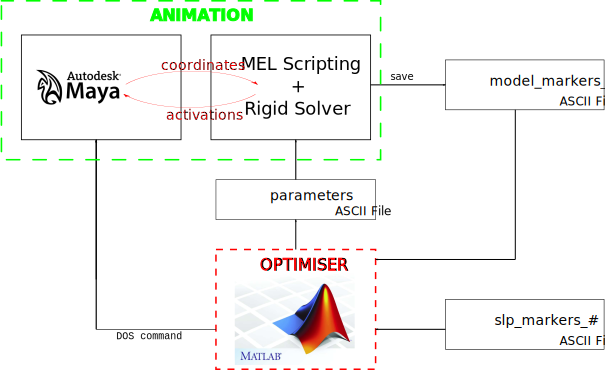
\includegraphics[width=\textwidth]{pics/implementation_schema}
	\caption[Implementation structure of the optimisation process]{\label{fig:implementation_schema}Implementation structure of the optimisation process.}
\end{figure}